%%%%%%%%%%%%%%%%%%%%%%%%%%%%%%%%%%%%%%%%%%%%%%%%%%%%%%
%SEC%%%%%%%%%%%%%%%%%%%%%%%%%%%%%%%%%%%%%%%%%%%%%%%%%%
\section{Detecção Facial}

%FRAME%%%%%%%%%%%%%%%%%%%%%%%%%%%%%%%%%%%%%%%%%%%%%%%
\begin{frame}{Definição}
O papel de um detector de faces é, dada uma imagem arbitrária, determinar se ela contém faces ou não e, caso positivo, retornar a localização e dimensões de cada face \cite{censtudy}
\end{frame}


%FRAME%%%%%%%%%%%%%%%%%%%%%%%%%%%%%%%%%%%%%%%%%%%%%%%
\begin{frame}{}
\begin{figure}[htbp]
    \caption{Fonte: \citeonline{nikons60ad}}
    \label{fig:nikon}
    \begin{center}
        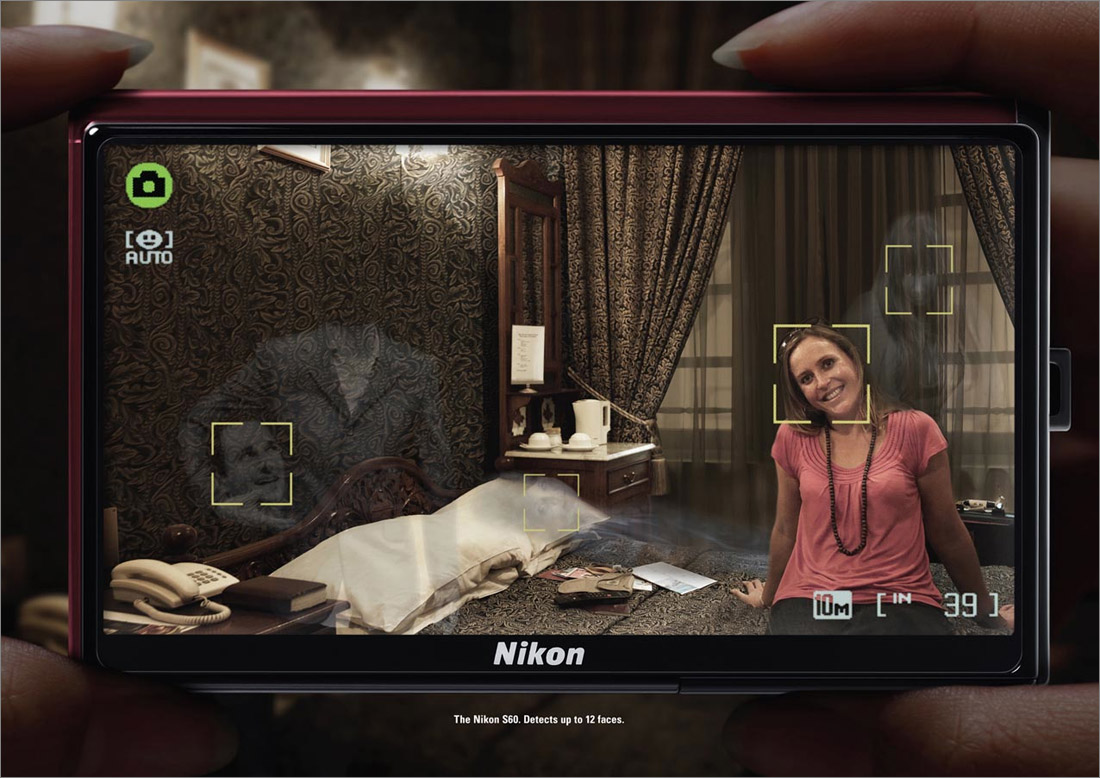
\includegraphics[width=0.9\linewidth]{imagens/nikon_s60_3.jpg}
    \end{center}
\end{figure}
\end{frame}


%FRAME%%%%%%%%%%%%%%%%%%%%%%%%%%%%%%%%%%%%%%%%%%%%%%%
%\begin{frame}{Métodos}
%\begin{figure}[htbp]
%    \label{fig:metodos_deteccao}
%    \begin{subfigure}[t]{0.45\textwidth}
%    \centering
%    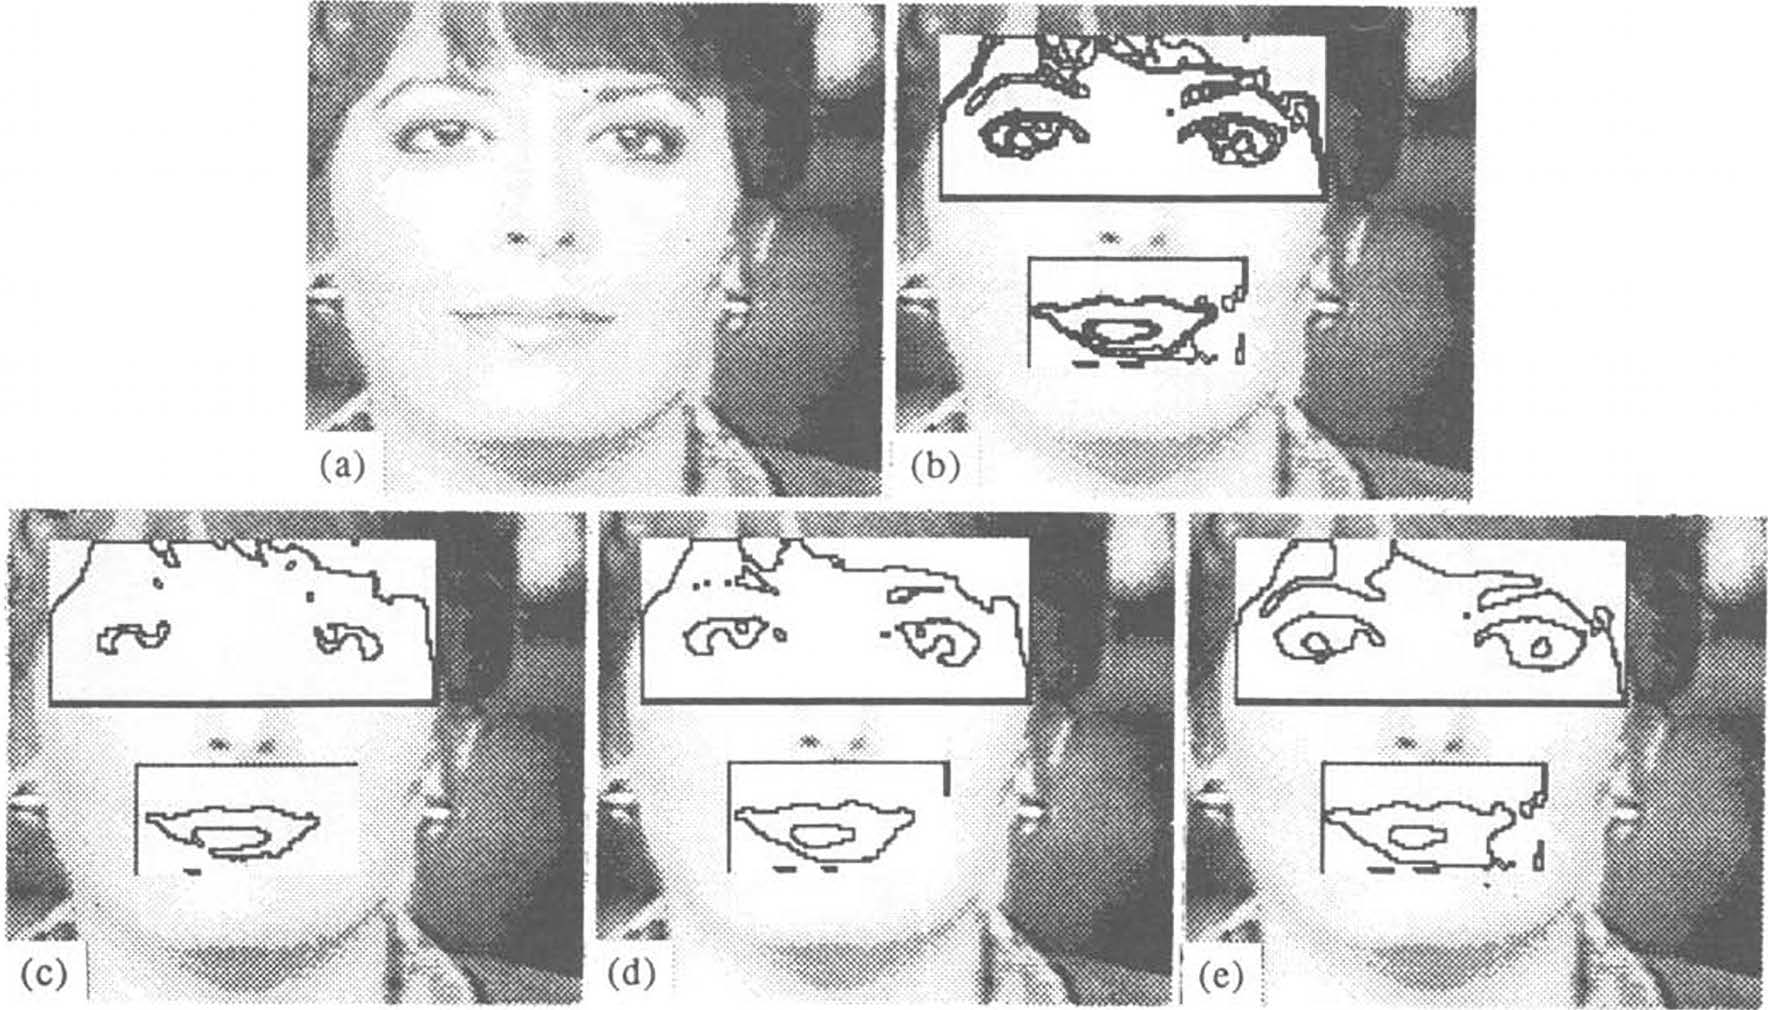
\includegraphics[width=0.7\textwidth]{imagens/yang_edge_detection.png}
%    \caption{Baseado em conhecimento. Fonte: \citeonline{yang1994human}}
%    \end{subfigure}
%    \hfill
%    \begin{subfigure}[t]{0.45\textwidth}
%    \centering
%    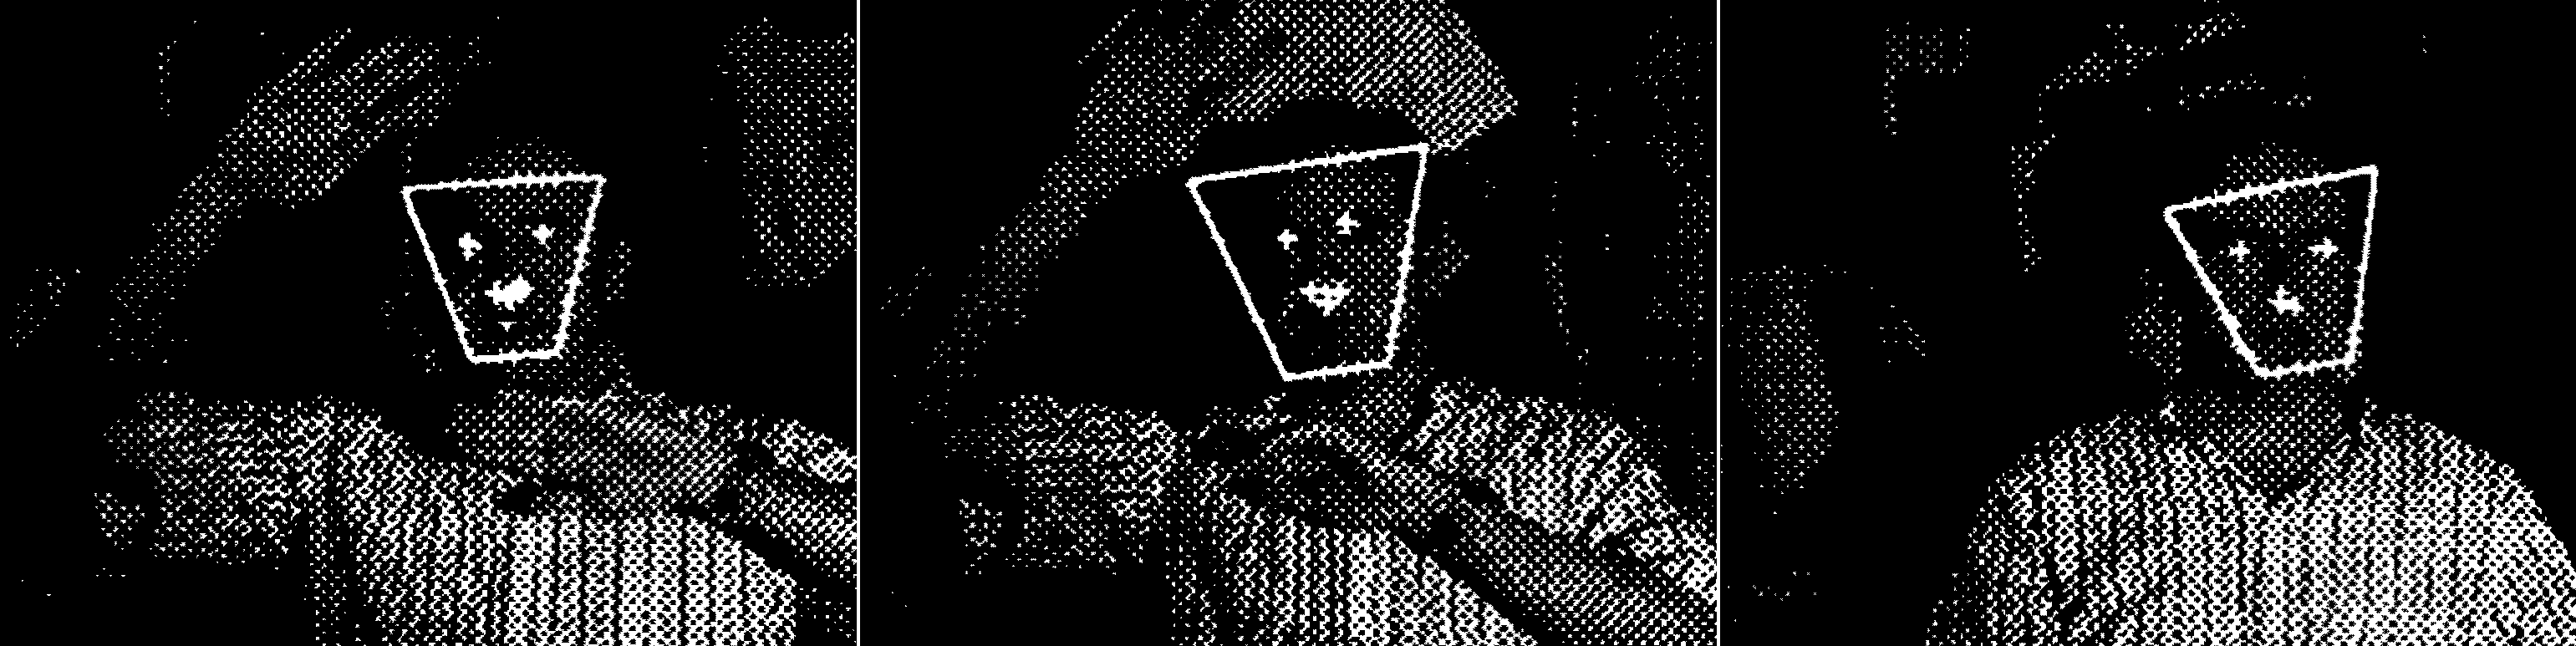
\includegraphics[width=0.7\textwidth]{imagens/leung.png}
%    \caption{Baseado em características invariantes.  Fonte: \citeonline{leung1995finding}}
%    \end{subfigure}
%    
%    \begin{subfigure}[t]{0.45\textwidth}
%    \centering
%    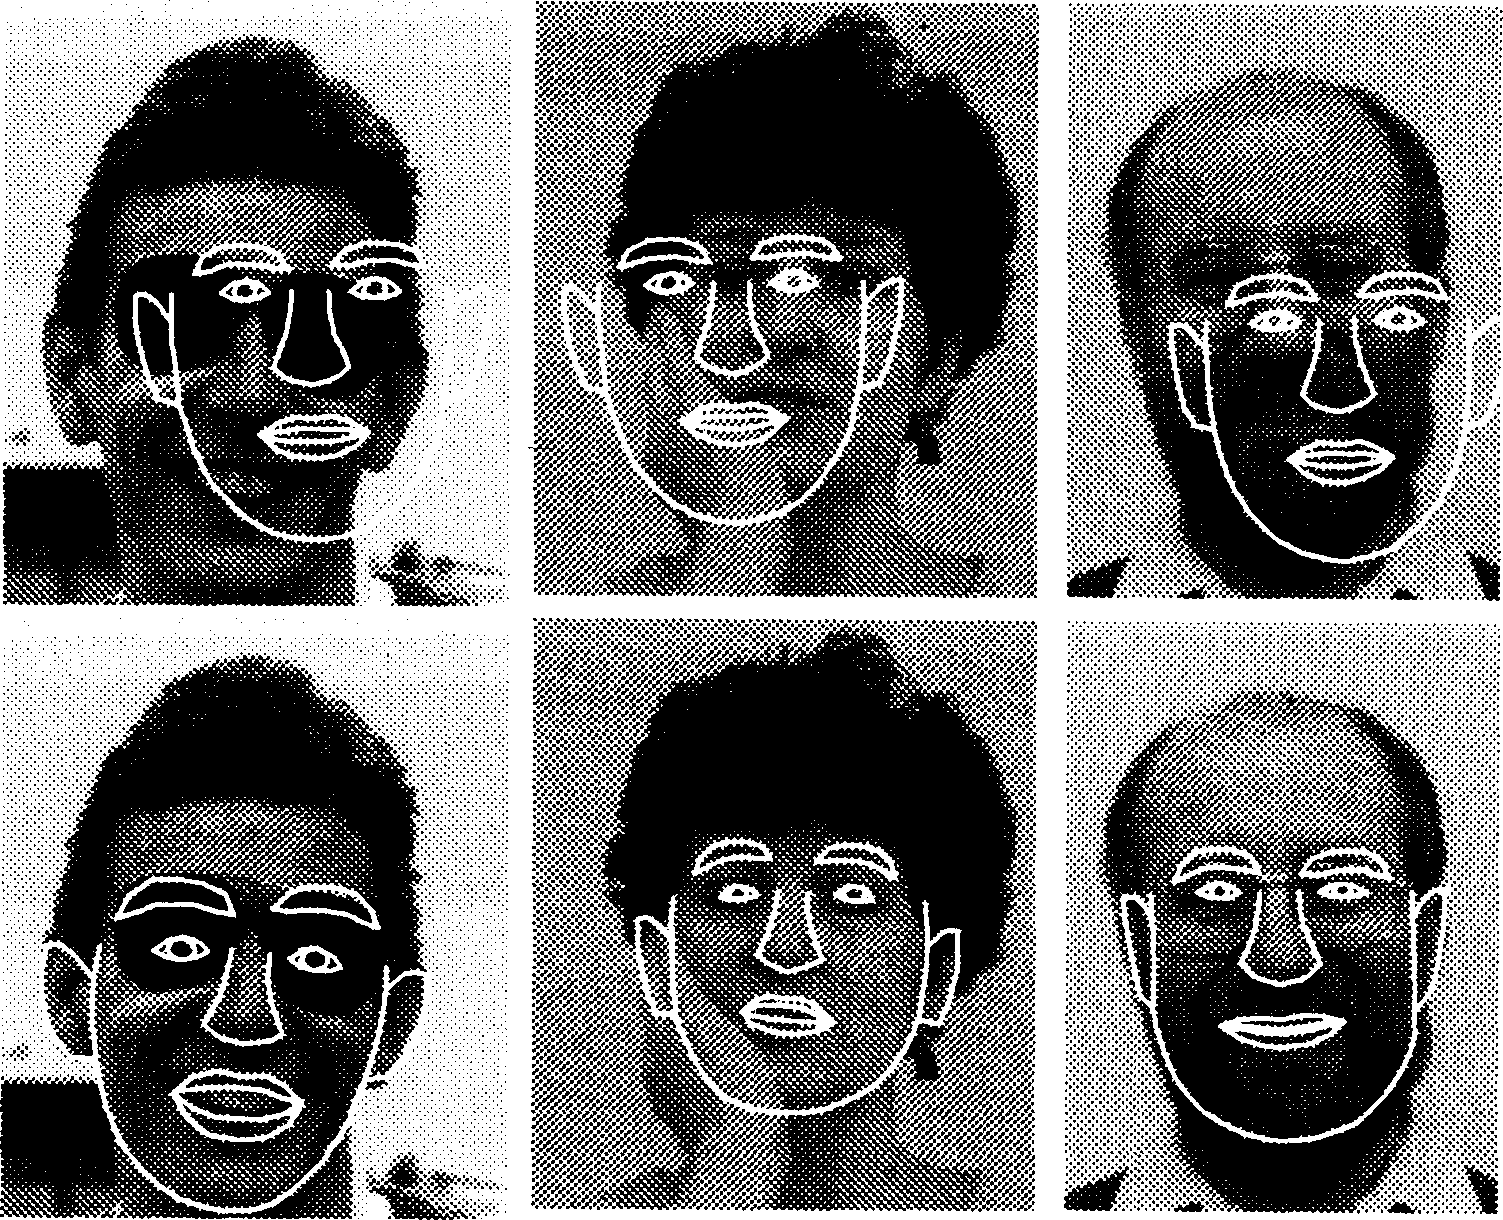
\includegraphics[width=0.6\textwidth]{imagens/lanitis_template.png}
%    \caption{Casamento de padrões. Fonte: \citeonline{lanitis1995automatic}}
%    \end{subfigure}
%    \hfill
%    \begin{subfigure}[t]{0.45\textwidth}
%    \centering
%    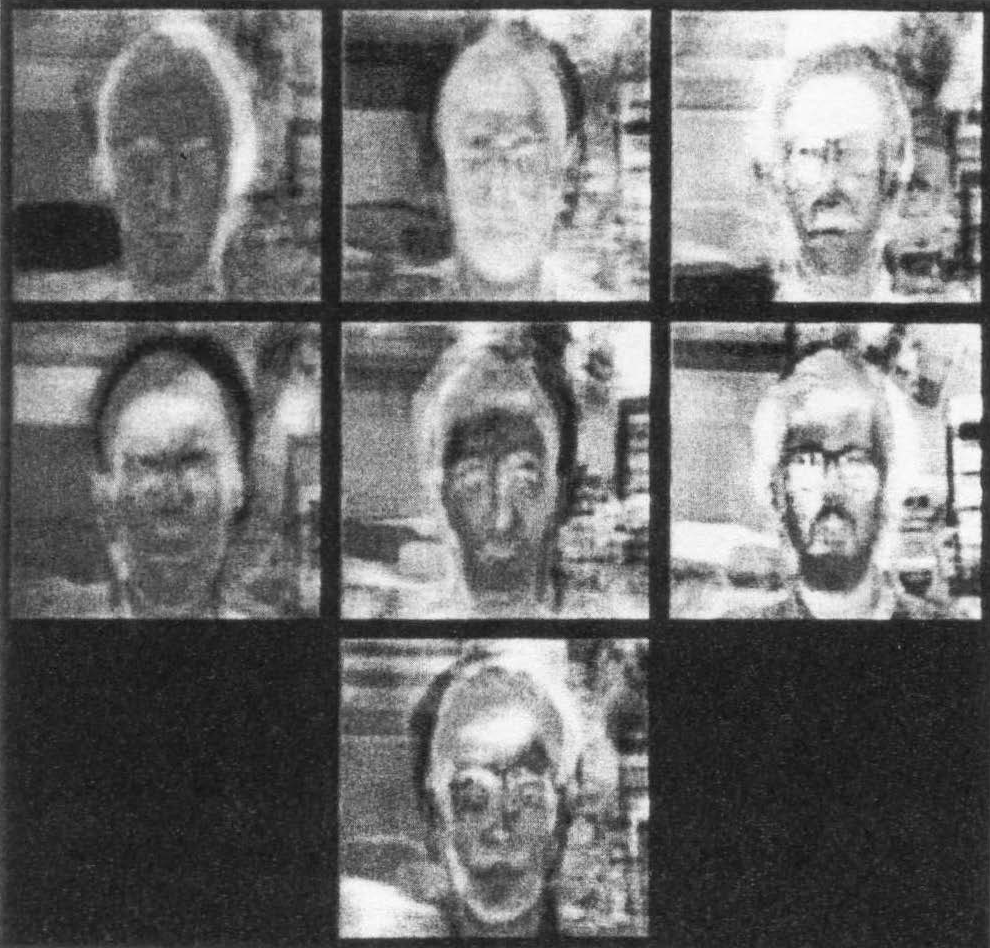
\includegraphics[width=0.6\textwidth]{imagens/turk_eigenfaces.png}
%    \caption{Baseado na aparência. Fonte: \citeonline{turk1991eigenfaces}}
%    \end{subfigure}
%\end{figure}
%\end{frame}


%FRAME%%%%%%%%%%%%%%%%%%%%%%%%%%%%%%%%%%%%%%%%%%%%%%%
\begin{frame}{Métodos}
\begin{itemize}
    \item Baseado em conhecimento
\end{itemize}

\begin{figure}[htbp]
    \centering
    \caption{Fonte: \citeonline{yang1994human}}
    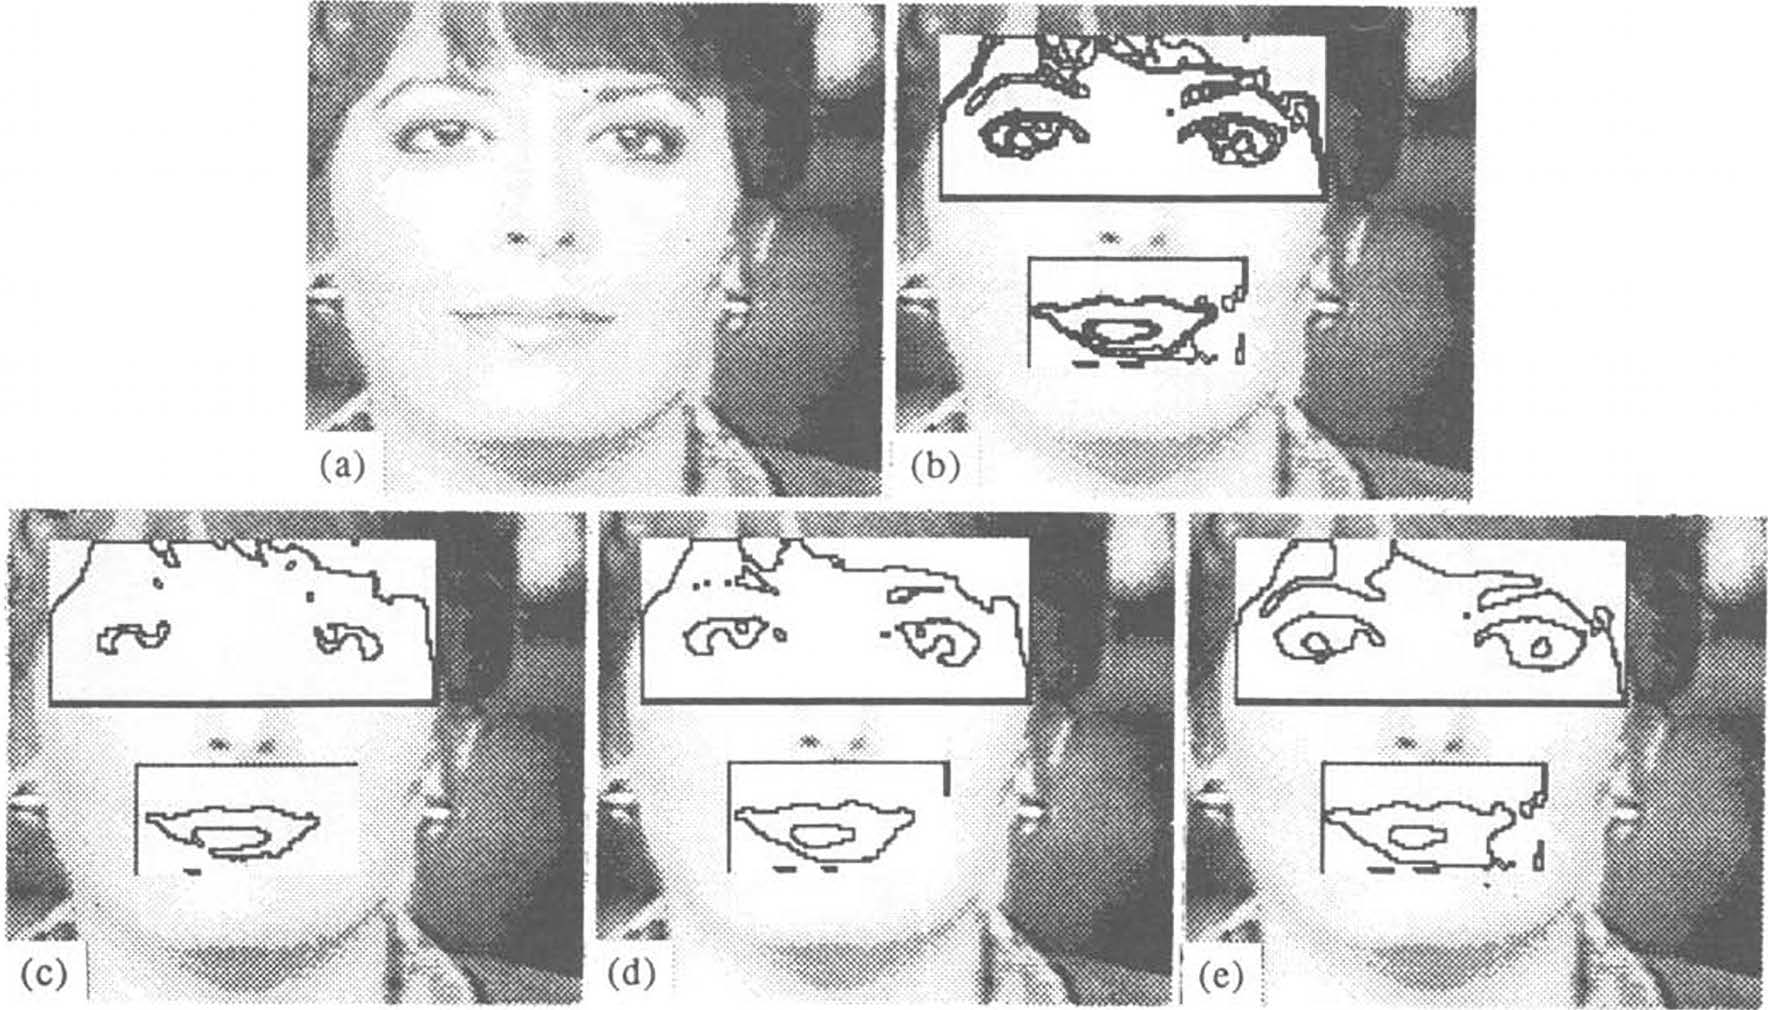
\includegraphics[height=0.6\textheight]{imagens/yang_edge_detection.png}
\end{figure}
\end{frame}


%FRAME%%%%%%%%%%%%%%%%%%%%%%%%%%%%%%%%%%%%%%%%%%%%%%%
\begin{frame}{Métodos}
\begin{itemize}
    \item Baseado em características invariantes
\end{itemize}

\begin{figure}[htbp]
    \caption{Fonte: \citeonline{leung1995finding}}
    \centering
    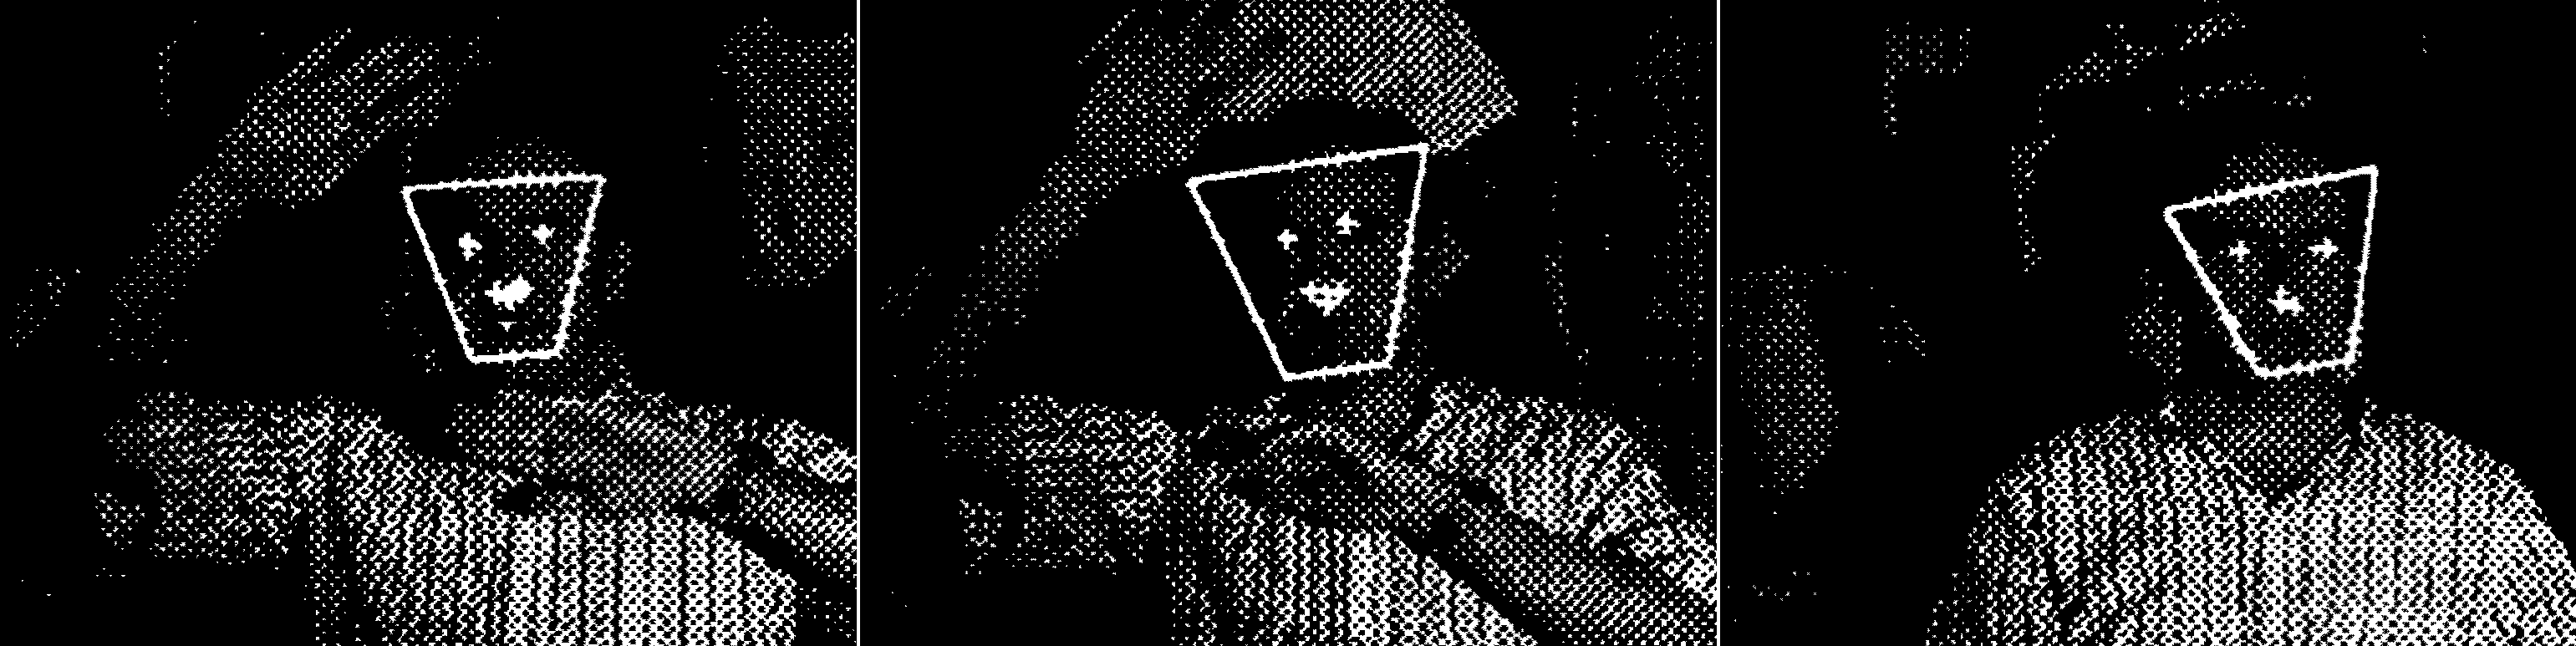
\includegraphics[height=0.6\textheight,width=\textwidth]{imagens/leung.png}
\end{figure}
\end{frame}


%FRAME%%%%%%%%%%%%%%%%%%%%%%%%%%%%%%%%%%%%%%%%%%%%%%%
\begin{frame}{Métodos}
\begin{itemize}
    \item Casamento de padrões
\end{itemize}

\begin{figure}[htbp]
    \caption{Fonte: \citeonline{lanitis1995automatic}}
    \centering
    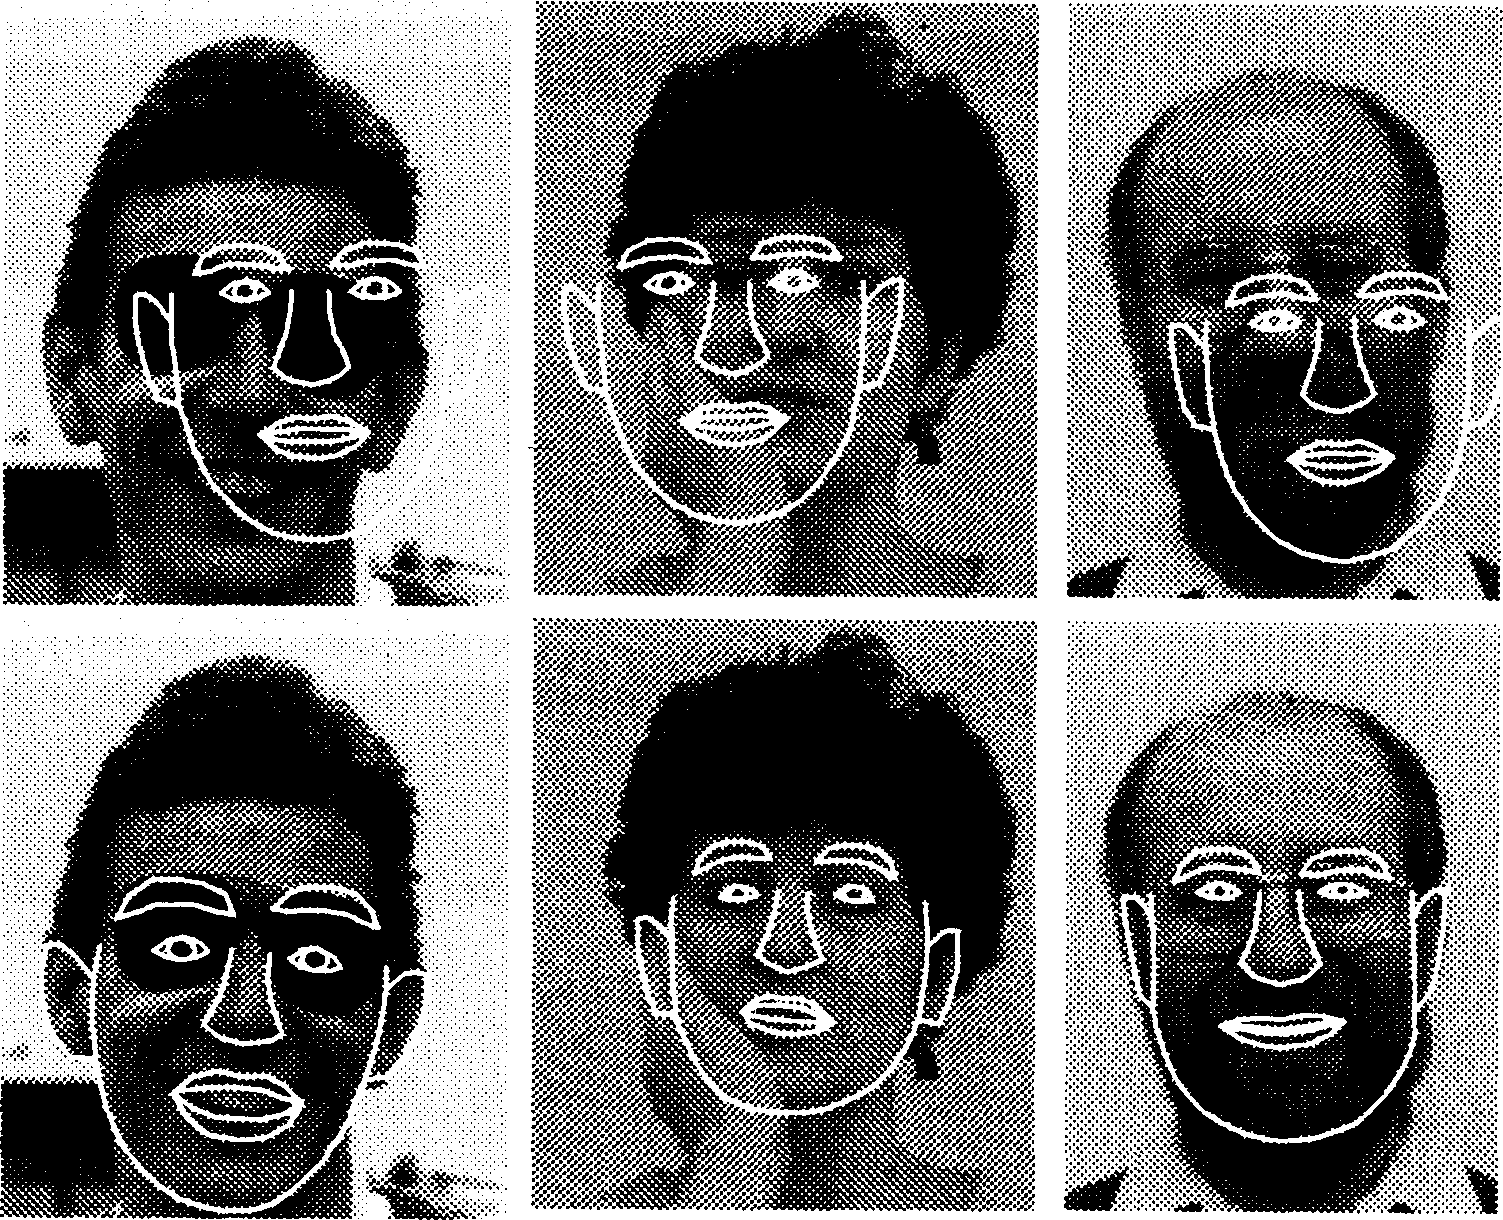
\includegraphics[height=0.6\textheight]{imagens/lanitis_template.png}
\end{figure}
\end{frame}


%FRAME%%%%%%%%%%%%%%%%%%%%%%%%%%%%%%%%%%%%%%%%%%%%%%%
\begin{frame}{Métodos}
\begin{itemize}
    \item Baseado na aparência
\end{itemize}

\begin{figure}
    \caption{Fonte: \citeonline{turk1991eigenfaces}}
    \centering
    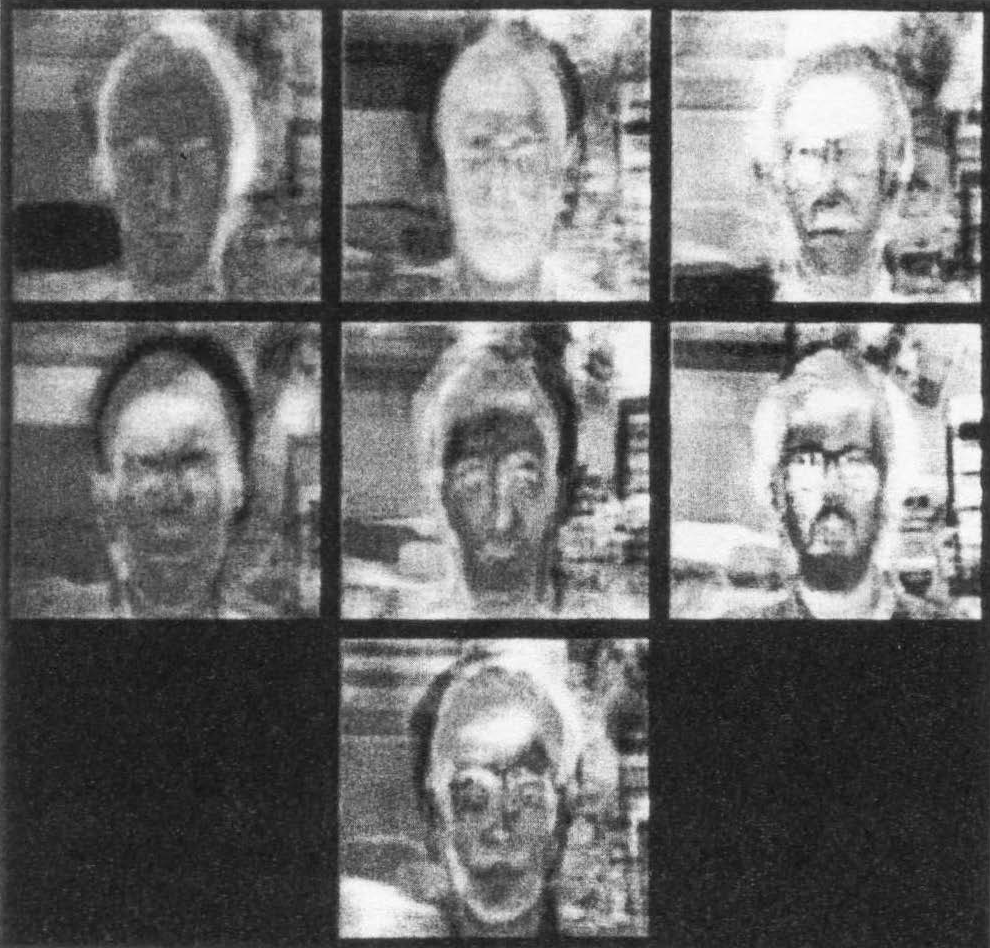
\includegraphics[height=0.6\textheight]{imagens/turk_eigenfaces.png}
\end{figure}
\end{frame}


%SUBSEC%%%%%%%%%%%%%%%%%%%%%%%%%%%%%%%%%%%%%%%%%%%%%%%
\subsection{Viola-Jones}

%FRAME%%%%%%%%%%%%%%%%%%%%%%%%%%%%%%%%%%%%%%%%%%%%%%%
\begin{frame}{Viola-Jones}
\begin{itemize}
    \item Algoritmo apresentado por Paul Viola e Michael Jones em 2001 \cite{Viola01rapidobject}
    \item Foi o primeiro método de detecção de faces em tempo real \citeonline{omaia2009sistema}
\end{itemize}
\end{frame}

%FRAME%%%%%%%%%%%%%%%%%%%%%%%%%%%%%%%%%%%%%%%%%%%%%%%
\begin{frame}{Viola-Jones}
\begin{itemize}
    \item Não é apenas para faces humanas
\end{itemize}

\begin{figure}
    \centering
    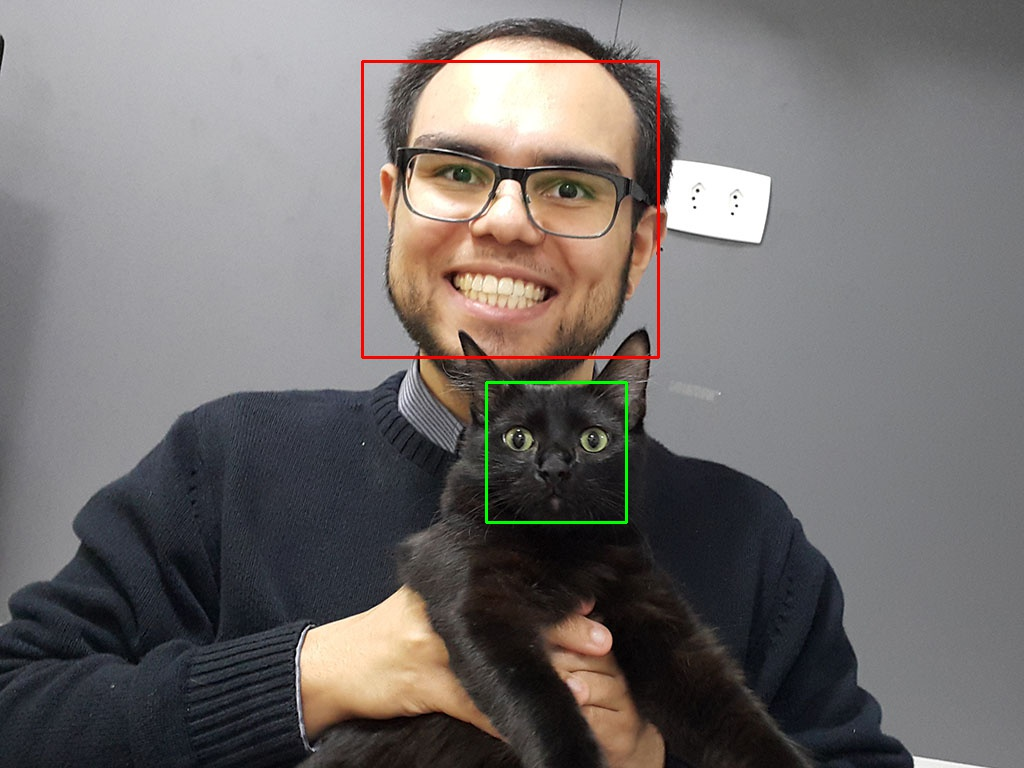
\includegraphics[width=0.8\textwidth]{imagens/detecta_joca.jpg}
\end{figure}
\end{frame}

%FRAME%%%%%%%%%%%%%%%%%%%%%%%%%%%%%%%%%%%%%%%%%%%%%%%
\begin{frame}{Viola-Jones}
Quatro estágios:
\medskip
\begin{itemize}
    \item Seleção de características Haar-like retangulares
    \item Criação da imagem integral
    \item Treino de classificadores por AdaBoost
    \item Uso de classificadores em cascata
\end{itemize}
\end{frame}


%SUBSEC%%%%%%%%%%%%%%%%%%%%%%%%%%%%%%%%%%%%%%%%%%%%%%%
\subsubsection{Características Haar}

%FRAME%%%%%%%%%%%%%%%%%%%%%%%%%%%%%%%%%%%%%%%%%%%%%%%
\begin{frame}{Características Haar}
\begin{itemize}
    \item Formadas por dois, três ou quatro retângulos
    \item O cálculo de uma única característica é bem simples: soma das intensidades dos pixels sob os retângulos pretos menos a soma dos valores sob os retângulos brancos
\end{itemize}

\begin{figure}
    \centering
    
\includegraphics[width=0.8\textwidth]{imagens/haar_like_features.png}
\end{figure}
\end{frame}

%FRAME%%%%%%%%%%%%%%%%%%%%%%%%%%%%%%%%%%%%%%%%%%%%%%%
\begin{frame}[fragile]{Características Haar}
\begin{itemize}
    \item Compara quão próximo o caso real está do caso ideal
\end{itemize}

\begin{figure}[h]
    \begin{adjustbox}{max width=\textwidth, max height=0.25\textheight}
    \begin{minipage}{0.45\textwidth}
    \centering
    \begin{tikzpicture}
    \matrix[square matrix, text=cyan] {
        0 & 0 &|[fill=black]| 1 &|[fill=black]| 1 \\
        0 & 0 &|[fill=black]| 1 &|[fill=black]| 1 \\
        0 & 0 &|[fill=black]| 1 &|[fill=black]| 1 \\
        0 & 0 &|[fill=black]| 1 &|[fill=black]| 1 \\
    };
    \end{tikzpicture}
    \caption{Intensidades ideais}
    \end{minipage}
    \begin{minipage}{0.1\textwidth}
    \centering
    $\vpointer$
    \end{minipage}
    \begin{minipage}{0.45\textwidth}
    \centering
    \begin{tikzpicture}
    \matrix[square matrix, text=cyan] {
        |[fill=black!20]|0.2 &|[fill=black!20]| 0.2 &|[fill=black!80]| 0.8 &|[fill=black!60]| 0.6 \\
        |[fill=black!10]|0.1 &|[fill=black!30]| 0.3 &|[fill=black!60]| 0.6 &|[fill=black!80]| 0.8 \\
        |[fill=black!20]|0.2 &|[fill=black!10]| 0.1 &|[fill=black!80]| 0.8 &|[fill=black!80]| 0.8 \\
        |[fill=black!20]|0.2 &|[fill=black!10]| 0.1 &|[fill=black!60]| 0.6 &|[fill=black!90]| 0.9 \\
    };
    \end{tikzpicture}
    \caption{Valores reais}
    \end{minipage}
    \end{adjustbox}
\end{figure}

\begin{align*}
\Delta  &= \frac{1}{n}  \sum_{preto}^{n} I(x) - \frac{1}{n}  \sum_{branco}^{n} I(x)\\
        &= 0,74 - 0,18 = 0,56 \nonumber
\end{align*}

\end{frame}


%FRAME%%%%%%%%%%%%%%%%%%%%%%%%%%%%%%%%%%%%%%%%%%%%%%%
\begin{frame}{Características Haar}
\begin{itemize}
    \item Características usadas para detectar olhos e nariz
\end{itemize}

\begin{figure}[htbp]
    \begin{subfigure}[c]{0.4\textwidth}
    \centering
    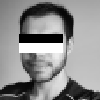
\includegraphics{imagens/julio_haar2.png}
    \end{subfigure}
    \begin{subfigure}[c]{0.4\textwidth}
    \centering
    
\includegraphics{imagens/julio_haar3.png}
    \end{subfigure}
\end{figure}
\end{frame}


%FRAME%%%%%%%%%%%%%%%%%%%%%%%%%%%%%%%%%%%%%%%%%%%%%%%
\begin{frame}{Características Haar}
Para cada subjanela de $24\times24$ pixels, seria necessário calcular 45396 características

\begin{center}{\huge Inviável!}\end{center}

\end{frame}


%SUBSUBSEC%%%%%%%%%%%%%%%%%%%%%%%%%%%%%%%%%%%%%%%%%%%%
\subsubsection{Imagem Integral}


%FRAME%%%%%%%%%%%%%%%%%%%%%%%%%%%%%%%%%%%%%%%%%%%%%%%
\begin{frame}{Imagem Integral}
\begin{itemize}
    \item Permite calcular as características em tempo constante
    \item É uma tabela onde cada elemento equivale à soma de todos os pixels à esquerda e acima do pixel atual
\end{itemize}

\begin{equation*} \label{eq:imagemintegral}
    ii(x,y) = \sum_{{x}'\leq x, {y}'\leq y} i({x}', {y}')
\end{equation*}

\end{frame}

%FRAME%%%%%%%%%%%%%%%%%%%%%%%%%%%%%%%%%%%%%%%%%%%%%%%
\begin{frame}[fragile]{Imagem Integral}

\begin{figure}[h]
    \begin{minipage}{0.44\textwidth}
    \caption{Imagem original}
    \centering
    \begin{adjustbox}{max width=\textwidth}
    \begin{tikzpicture}
    \matrix[square matrix] {
        0.1 & 0.1 & 0.2 & 0.1 & 0.7 & 0.1 \\
        0.2 & 0.3 & 0.2 & 0.7 & 0.8 & 0.2 \\
        0.1 & 0.4 & 0.3 & 0.3 & 0.1 & 0.3 \\
        0.1 & 0.5 & 0.1 & 0.1 & 0.2 & 0.8 \\
        0.1 & 0.4 & 0.8 & 0.5 & 0.6 & 0.5\\
    };
    \end{tikzpicture}
    \end{adjustbox}
    \end{minipage}
    \begin{minipage}{0.1\textwidth}
    \caption{ }
    \centering
    $\vpointer$
    \end{minipage}
    \begin{minipage}{0.44\textwidth}
    \caption{Imagem integral}
    \centering
    \begin{adjustbox}{max width=\textwidth}
    \begin{tikzpicture}
    \matrix[square matrix] {
        0.1 & 0.2 & 0.4 & 0.5 & 1.2 & 1.3 \\
        0.3 & 0.7 & 1.1 & 1.9 & 3.4 & 3.7 \\
        0.4 & 1.2 & 1.9 & 3.0 & 4.6 & 5.2 \\
        0.5 & 1.7 & 2.5 & 3.7 & 5.3 & 6.7 \\
        0.6 & 2.3 & 3.9 & 5.6 & 8.0 & 9.9 \\
    };
    \end{tikzpicture}
    \end{adjustbox}
    \end{minipage}
\end{figure}

\end{frame}


%FRAME%%%%%%%%%%%%%%%%%%%%%%%%%%%%%%%%%%%%%%%%%%%%%%%
\begin{frame}[fragile]{Imagem Integral}

\begin{figure}[h]
    \begin{minipage}{0.44\textwidth}
    \caption{Imagem original}
    \centering
    \begin{adjustbox}{max width=\textwidth}
    \begin{tikzpicture}
    \matrix[square matrix, opacity=0.2] (m){
        0.1 & 0.1 & 0.2 & 0.1 & 0.7 & 0.1 \\
        0.2 & 0.3 & 0.2 & 0.7 & 0.8 & 0.2 \\
        0.1 & 0.4 & 0.3 & 0.3 & 0.1 & 0.3 \\
        0.1 & 0.5 & 0.1 & 0.1 & 0.2 & 0.8 \\
        0.1 & 0.4 & 0.8 & 0.5 & 0.6 & 0.5 \\
    };
    \filldraw[fill=black!50, fill opacity=0.2, text opacity=1] (m-1-1.north west) rectangle (m-1-2.south east) node[pos=.5] {A};
    \filldraw[fill=black!70, fill opacity=0.2, text opacity=1] (m-1-3.north west) rectangle (m-1-4.south east) node[pos=.5] {B};
    \filldraw[fill=black!90, fill opacity=0.2, text opacity=1] (m-2-1.north west) rectangle (m-4-2.south east) node[pos=.5] {C};
    \filldraw[fill=yellow, fill opacity=0.2, text opacity=1] (m-2-3.north west) rectangle (m-4-4.south east) node[pos=.5] {D};
    
    \fill[blue] (m-1-2.south east) circle(2pt) node[above right] {P1};
    \fill[blue] (m-1-4.south east) circle(2pt) node[above right] {P2};
    \fill[blue] (m-4-2.south east) circle(2pt) node[above right] {P3};
    \fill[blue] (m-4-4.south east) circle(2pt) node[above right] {P4};
    \end{tikzpicture}
    \end{adjustbox}
    \end{minipage}
    \begin{minipage}{0.1\textwidth}
    \caption{ }
    \centering
    $\vpointer$
    \end{minipage}
    \begin{minipage}{0.44\textwidth}
    \caption{Imagem integral}
    \centering
    \begin{adjustbox}{max width=\textwidth}
    \begin{tikzpicture}
    \matrix[square matrix] (m){
        0.1 & 0.2 & 0.4 & 0.5 & 1.2 & 1.3 \\
        0.3 & 0.7 & 1.1 & 1.9 & 3.4 & 3.7 \\
        0.4 & 1.2 & 1.9 & 3.0 & 4.6 & 5.2 \\
        0.5 & 1.7 & 2.5 & 3.7 & 5.3 & 6.7 \\
        0.6 & 2.3 & 3.9 & 5.6 & 8.0 & 9.9 \\
    };
    \filldraw[fill=yellow, fill opacity=0.2] (m-1-2.north west) rectangle (m-1-2.south east);
    \filldraw[fill=yellow, fill opacity=0.2] (m-1-4.north west) rectangle (m-1-4.south east);
    \filldraw[fill=yellow, fill opacity=0.2] (m-4-2.north west) rectangle (m-4-2.south east);
    \filldraw[fill=yellow, fill opacity=0.2] (m-4-4.north west) rectangle (m-4-4.south east);
    \draw[blue,<-,shorten <=1pt] (m-1-2)
    |- +(0.2,0.8)
    node[right] {$ii(P1)$};
     \draw[blue,<-,shorten <=1pt] (m-1-4)
    |- +(0.2,0.8)
    node[right] {$ii(P2)$};
    \draw[blue,<-,shorten <=1pt] (m-4-2)
    |- +(0.2,-1.4)
    node[right] {$ii(P3)$};
    \draw[blue,<-,shorten <=1pt] (m-4-4)
    |- +(0.2,-1.4)
    node[right] {$ii(P4)$};
    \end{tikzpicture}%
    \end{adjustbox}
    \end{minipage}
\end{figure}

\begin{align*}
D &= (ii(P4) + ii(P1)) - (ii(P2) + ii(P3)) \\
  &= (3,7 + 02) - (0,5 + 1,7) = 1,7 \nonumber
\end{align*}

\end{frame}



%FRAME%%%%%%%%%%%%%%%%%%%%%%%%%%%%%%%%%%%%%%%%%%%%%%%
%\begin{frame}[fragile]{Imagem Integral}
%
%Cálculo da área em amarelo
%
%\begin{figure}[h]
%    \begin{minipage}{0.44\textwidth}
%    \caption{Imagem original}
%    \centering
%    \begin{adjustbox}{max width=\textwidth}
%    \begin{tikzpicture}
%    \matrix[square matrix] {
%        |[fill=yellow!25]|0.1 & |[fill=yellow!25]|0.1 & 0.2 & 0.1 & 0.7 & 0.1 \\
%        |[fill=yellow!25]|0.2 & |[fill=yellow!25]|0.3 & 0.2 & 0.7 & 0.8 & 0.2 \\
%        |[fill=yellow!25]|0.1 & |[fill=yellow!25]|0.4 & 0.3 & 0.3 & 0.1 & 0.3 \\
%        0.1 & 0.5 & 0.1 & 0.1 & 0.2 & 0.8 \\
%        0.1 & 0.4 & 0.8 & 0.5 & 0.6 & 0.5\\
%    };
%    \end{tikzpicture}
%    \end{adjustbox}
%    \end{minipage}
%    \begin{minipage}{0.1\textwidth}
%    \caption{ }
%    \centering
%    $\vpointer$
%    \end{minipage}
%    \begin{minipage}{0.44\textwidth}
%    \caption{Imagem integral}
%    \centering
%    \begin{adjustbox}{max width=\textwidth}
%    \begin{tikzpicture}
%    \matrix[square matrix] {
%        0.1 & 0.2 & 0.4 & 0.5 & 1.2 & 1.3 \\
%        0.3 & 0.7 & 1.1 & 1.9 & 3.4 & 3.7 \\
%        0.4 &|[fill=yellow!25]| 1.2 & 1.9 & 3.0 & 4.6 & 5.2 \\
%        0.5 & 1.7 & 2.5 & 3.7 & 5.3 & 6.7 \\
%        0.6 & 2.3 & 3.9 & 5.6 & 8.0 & 9.9 \\
%    };
%    \end{tikzpicture}
%    \end{adjustbox}
%    \end{minipage}
%\end{figure}
%
%\end{frame}


%FRAME%%%%%%%%%%%%%%%%%%%%%%%%%%%%%%%%%%%%%%%%%%%%%%%
\begin{frame}[fragile]{Imagem Integral}

\begin{figure}[h]
    \begin{minipage}{0.44\textwidth}
    \caption{Imagem original}
    \centering
    \begin{adjustbox}{max width=\textwidth}
    \begin{tikzpicture}
    \matrix[square matrix] {
        |[fill=yellow!25]|0.1 & |[fill=yellow!25]|0.1 & |[fill=yellow!25]|0.2 &|[fill=yellow!25]| 0.1 & 0.7 & 0.1 \\
        |[fill=yellow!25]|0.2 & |[fill=yellow!25]|0.3 & |[fill=yellow!25]|0.2 & |[fill=yellow!25]|0.7 & 0.8 & 0.2 \\
        |[fill=yellow!25]|0.1 & |[fill=yellow!25]|0.4 & |[fill=yellow!25]|0.3 & |[fill=yellow!25]|0.3 & 0.1 & 0.3 \\
        |[fill=yellow!25]|0.1 & |[fill=yellow!25]|0.5 & |[fill=yellow!25]|0.1 & |[fill=yellow!25]|0.1 & 0.2 & 0.8 \\
        0.1 & 0.4 & 0.8 & 0.5 & 0.6 & 0.5\\
    };
    \end{tikzpicture}
    \end{adjustbox}
    \end{minipage}
    \begin{minipage}{0.1\textwidth}
    \caption{ }
    \centering
    $\vpointer$
    \end{minipage}
    \begin{minipage}{0.44\textwidth}
    \caption{Imagem integral}
    \centering
    \begin{adjustbox}{max width=\textwidth}
    \begin{tikzpicture}
    \matrix[square matrix] {
        0.1 & 0.2 & 0.4 & 0.5 & 1.2 & 1.3 \\
        0.3 & 0.7 & 1.1 & 1.9 & 3.4 & 3.7 \\
        0.4 & 1.2 & 1.9 & 3.0 & 4.6 & 5.2 \\
        0.5 & 1.7 & 2.5 &|[fill=yellow!25]|3.7 & 5.3 & 6.7 \\
        0.6 & 2.3 & 3.9 & 5.6 & 8.0 & 9.9 \\
    };
    \end{tikzpicture}
    \end{adjustbox}
    \end{minipage}
\end{figure}

\end{frame}


%FRAME%%%%%%%%%%%%%%%%%%%%%%%%%%%%%%%%%%%%%%%%%%%%%%%
\begin{frame}[fragile]{Imagem Integral}

\begin{figure}[h]
    \begin{minipage}{0.44\textwidth}
    \caption{Imagem original}
    \centering
    \begin{adjustbox}{max width=\textwidth}
    \begin{tikzpicture}
    \matrix[square matrix] {
        |[fill=red!25]|0.1 & |[fill=red!25]|0.1 & |[fill=red!25]|0.2 &|[fill=red!25]| 0.1 & 0.7 & 0.1 \\
        |[fill=yellow!25]|0.2 & |[fill=yellow!25]|0.3 & |[fill=yellow!25]|0.2 & |[fill=yellow!25]|0.7 & 0.8 & 0.2 \\
        |[fill=yellow!25]|0.1 & |[fill=yellow!25]|0.4 & |[fill=yellow!25]|0.3 & |[fill=yellow!25]|0.3 & 0.1 & 0.3 \\
        |[fill=yellow!25]|0.1 & |[fill=yellow!25]|0.5 & |[fill=yellow!25]|0.1 & |[fill=yellow!25]|0.1 & 0.2 & 0.8 \\
        0.1 & 0.4 & 0.8 & 0.5 & 0.6 & 0.5\\
    };
    \end{tikzpicture}
    \end{adjustbox}
    \end{minipage}
    \begin{minipage}{0.1\textwidth}
    \caption{ }
    \centering
    $\vpointer$
    \end{minipage}
    \begin{minipage}{0.44\textwidth}
    \caption{Imagem integral}
    \centering
    \begin{adjustbox}{max width=\textwidth}
    \begin{tikzpicture}
    \matrix[square matrix] {
        0.1 & 0.2 & 0.4 &|[fill=red!25]| 0.5 & 1.2 & 1.3 \\
        0.3 & 0.7 & 1.1 & 1.9 & 3.4 & 3.7 \\
        0.4 & 1.2 & 1.9 & 3.0 & 4.6 & 5.2 \\
        0.5 & 1.7 & 2.5 &|[fill=yellow!25]|3.7 & 5.3 & 6.7 \\
        0.6 & 2.3 & 3.9 & 5.6 & 8.0 & 9.9 \\
    };
    \end{tikzpicture}
    \end{adjustbox}
    \end{minipage}
\end{figure}

\end{frame}


%FRAME%%%%%%%%%%%%%%%%%%%%%%%%%%%%%%%%%%%%%%%%%%%%%%%
\begin{frame}[fragile]{Imagem Integral}

\begin{figure}[h]
    \begin{minipage}{0.44\textwidth}
    \caption{Imagem original}
    \centering
    \begin{adjustbox}{max width=\textwidth}
    \begin{tikzpicture}
    \matrix[square matrix] {
        |[fill=red!50]|0.1 & |[fill=red!50]|0.1 & |[fill=red!25]|0.2 &|[fill=red!25]| 0.1 & 0.7 & 0.1 \\
        |[fill=red!25]|0.2 & |[fill=red!25]|0.3 & |[fill=yellow!25]|0.2 & |[fill=yellow!25]|0.7 & 0.8 & 0.2 \\
        |[fill=red!25]|0.1 & |[fill=red!25]|0.4 & |[fill=yellow!25]|0.3 & |[fill=yellow!25]|0.3 & 0.1 & 0.3 \\
        |[fill=red!25]|0.1 & |[fill=red!25]|0.5 & |[fill=yellow!25]|0.1 & |[fill=yellow!25]|0.1 & 0.2 & 0.8 \\
        0.1 & 0.4 & 0.8 & 0.5 & 0.6 & 0.5\\
    };
    \end{tikzpicture}
    \end{adjustbox}
    \end{minipage}
    \begin{minipage}{0.1\textwidth}
    \caption{ }
    \centering
    $\vpointer$
    \end{minipage}
    \begin{minipage}{0.44\textwidth}
    \caption{Imagem integral}
    \centering
    \begin{adjustbox}{max width=\textwidth}
    \begin{tikzpicture}
    \matrix[square matrix] {
        0.1 & 0.2 & 0.4 &|[fill=red!25]| 0.5 & 1.2 & 1.3 \\
        0.3 & 0.7 & 1.1 & 1.9 & 3.4 & 3.7 \\
        0.4 & 1.2 & 1.9 & 3.0 & 4.6 & 5.2 \\
        0.5 &|[fill=red!25]|1.7 & 2.5 &|[fill=yellow!25]|3.7 & 5.3 & 6.7 \\
        0.6 & 2.3 & 3.9 & 5.6 & 8.0 & 9.9 \\
    };
    \end{tikzpicture}
    \end{adjustbox}
    \end{minipage}
\end{figure}

\end{frame}


%FRAME%%%%%%%%%%%%%%%%%%%%%%%%%%%%%%%%%%%%%%%%%%%%%%%
\begin{frame}[fragile]{Imagem Integral}

\begin{figure}[h]
    \begin{minipage}{0.44\textwidth}
    \caption{Imagem original}
    \centering
    \begin{adjustbox}{max width=\textwidth}
    \begin{tikzpicture}
    \matrix[square matrix] {
        |[fill=red!25]|0.1 & |[fill=red!25]|0.1 & |[fill=red!25]|0.2 &|[fill=red!25]| 0.1 & 0.7 & 0.1 \\
        |[fill=red!25]|0.2 & |[fill=red!25]|0.3 & |[fill=yellow!25]|0.2 & |[fill=yellow!25]|0.7 & 0.8 & 0.2 \\
        |[fill=red!25]|0.1 & |[fill=red!25]|0.4 & |[fill=yellow!25]|0.3 & |[fill=yellow!25]|0.3 & 0.1 & 0.3 \\
        |[fill=red!25]|0.1 & |[fill=red!25]|0.5 & |[fill=yellow!25]|0.1 & |[fill=yellow!25]|0.1 & 0.2 & 0.8 \\
        0.1 & 0.4 & 0.8 & 0.5 & 0.6 & 0.5\\
    };
    \end{tikzpicture}
    \end{adjustbox}
    \end{minipage}
    \begin{minipage}{0.1\textwidth}
    \caption{ }
    \centering
    $\vpointer$
    \end{minipage}
    \begin{minipage}{0.44\textwidth}
    \caption{Imagem integral}
    \centering
    \begin{adjustbox}{max width=\textwidth}
    \begin{tikzpicture}
    \matrix[square matrix] {
        0.1 & |[fill=yellow!25]|0.2 & 0.4 &|[fill=red!25]| 0.5 & 1.2 & 1.3 \\
        0.3 & 0.7 & 1.1 & 1.9 & 3.4 & 3.7 \\
        0.4 & 1.2 & 1.9 & 3.0 & 4.6 & 5.2 \\
        0.5 &|[fill=red!25]|1.7 & 2.5 &|[fill=yellow!25]|3.7 & 5.3 & 6.7 \\
        0.6 & 2.3 & 3.9 & 5.6 & 8.0 & 9.9 \\
    };
    \end{tikzpicture}
    \end{adjustbox}
    \end{minipage}
\end{figure}
\end{frame}


%SUBSEC%%%%%%%%%%%%%%%%%%%%%%%%%%%%%%%%%%%%%%%%%%%%%%%
\subsubsection{AdaBoost}

%FRAME%%%%%%%%%%%%%%%%%%%%%%%%%%%%%%%%%%%%%%%%%%%%%%%
\begin{frame}{AdaBoost}
\begin{itemize}
    \item Mesmo usando a imagem integral, calcular todas as características continua inviável
    \item É possível formar um classificador eficiente usando apenas as \textbf{características mais relevantes}. Elas podem ser selecionadas pelo algoritmo de aprendizado de máquina AdaBoost
\end{itemize}
\end{frame}


%FRAME%%%%%%%%%%%%%%%%%%%%%%%%%%%%%%%%%%%%%%%%%%%%%%%
\begin{frame}{AdaBoost}
\begin{itemize}
    \item \textbf{Ada}ptive \textbf{Boost}
    \item Combina, de forma ponderada, classificadores fracos para obter um classificador forte
\end{itemize}

\begin{equation*} \label{eq:adaboost}
    \tikzmark{a1}F\tikzmark{a2}(\tikzmark{b1}x\tikzmark{b2}) = \tikzmark{c1}\alpha_1\tikzmark{c2}\tikzmark{d1}f_1\tikzmark{d2}(x) + \alpha_2f_2(x) + \alpha_3f_3(x) \ldots
\end{equation*}

\begin{tikzpicture}[remember picture,overlay]

%\draw[decorate,decoration={brace,mirror}]
%  (pic cs:a1) -- node (aux) {} (pic cs:a2);
\node (aux) at ($(pic cs:a1)!0.5!(pic cs:a2)$) {};
\draw[->,>=latex]
  (aux) |-
  ++(10pt,-60pt) 
  node[right] 
    {classificador forte};

%\draw[decorate,decoration={brace,mirror}]
%  (pic cs:b1) -- node (aux) {} (pic cs:b2);
\node (aux) at ($(pic cs:b1)!0.5!(pic cs:b2)$) {};
\draw[->,>=latex]
  (aux) |-
  ++(10pt,-45pt) 
  node[right] 
    {imagem};
    
%\draw[decorate,decoration={brace,mirror}]
%  (pic cs:c1) -- node (aux) {} (pic cs:c2);
\node (aux) at ($(pic cs:c1)!0.5!(pic cs:c2)$) {};
\draw[->,>=latex]
  (aux) |-
  ++(10pt,-30pt) 
  node[right] 
    {peso};
    
%\draw[decorate,decoration={brace,mirror}]
%  (pic cs:d1) -- node (aux) {} (pic cs:d2);
\node (aux) at ($(pic cs:d1)!0.5!(pic cs:d2)$) {};
\draw[->,>=latex]
  (aux) |-
  ++(10pt,-15pt) 
  node[right] 
    {classificador fraco};
\end{tikzpicture}

\end{frame}

%FRAME%%%%%%%%%%%%%%%%%%%%%%%%%%%%%%%%%%%%%%%%%%%%%%%
\begin{frame}{AdaBoost}
Algoritmo:
\medskip
\begin{itemize}
    \item Inicia com pesos iguais para todas as imagens de treino
    \item Em cada iteração, encontra o classificador fraco com menor erro e aumenta o peso dos exemplos classificados erroneamente
    \item Calcula o classificador forte como uma combinação linear dos classificadores fracos
\end{itemize}
\end{frame}


%FRAME%%%%%%%%%%%%%%%%%%%%%%%%%%%%%%%%%%%%%%%%%%%%%%%
\begin{frame}{AdaBoost}
\begin{itemize}
    \item Classificador com 200 características:
        \begin{itemize}
            \item 95\% de detecção
            \item 1 falso-positivo em 14084 ($1,4\times10^{-4}$ FPR)
            \item 1,43 FPS (0,7 segundos para $384\times288$ pixels)
        \end{itemize}
\end{itemize}

\begin{center}
\begin{tikzpicture}
    \node[anchor=south west,inner sep=0] (image) at (0,0) {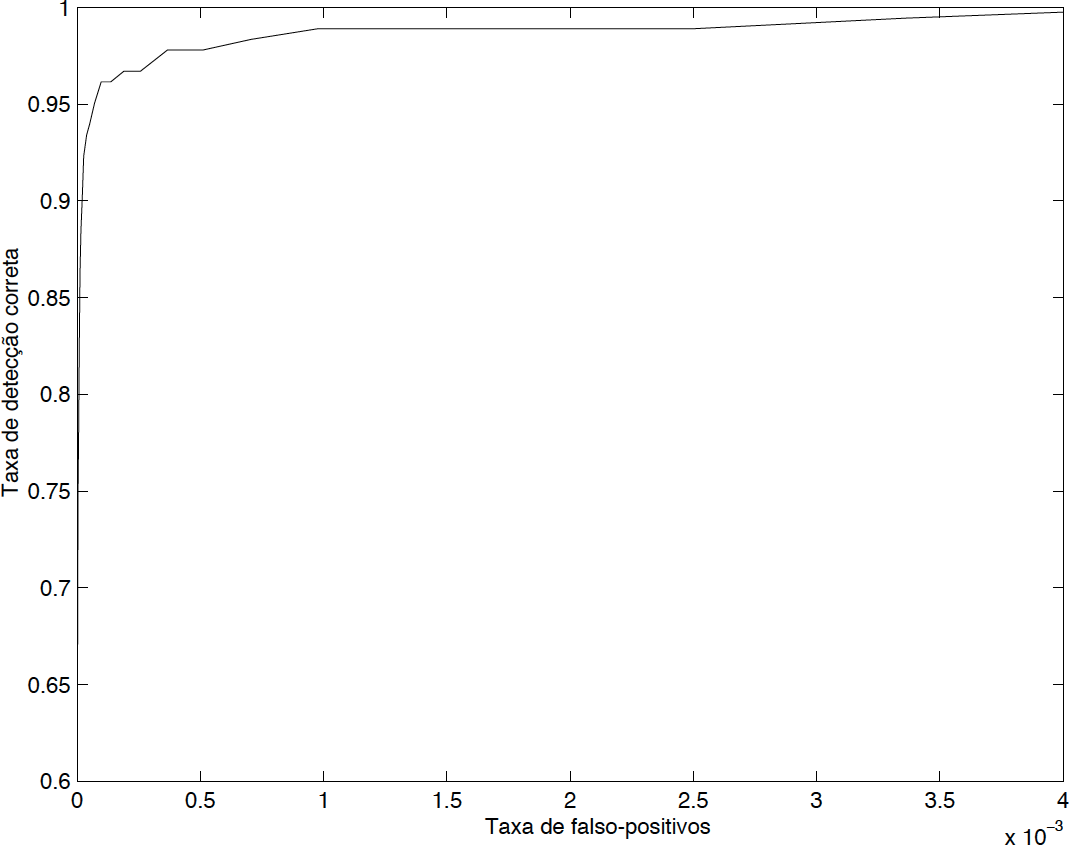
\includegraphics[height=0.6\textheight,width=0.8\textwidth]{imagens/roc_200_features.png}};
    \begin{scope}[x={(image.south east)},y={(image.north west)}]
        %\draw[help lines,xstep=.1,ystep=.1] (0,0) grid (1,1);
        %\foreach \x in {0,1,...,9} { \node [anchor=north] at (\x/10,0) {0.\x}; }
        %\foreach \y in {0,1,...,9} { \node [anchor=east] at (0,\y/10) {0.\y}; }
        \draw[red] (0.6,0.6) node {Não é bom o suficiente!};
        \draw[red] (0.6,0.4) node {Nem tempo real};
    \end{scope}
\end{tikzpicture}
\end{center}

\end{frame}


%SUBSEC%%%%%%%%%%%%%%%%%%%%%%%%%%%%%%%%%%%%%%%%%%%%%%%
\subsubsection{Classificadores em Cascata}

%FRAME%%%%%%%%%%%%%%%%%%%%%%%%%%%%%%%%%%%%%%%%%%%%%%%
\begin{frame}[fragile]{Classificadores em Cascata}
\begin{itemize}
    \item Gasta tempo apenas com faces em potencial
    \item Classificador de duas características: quase 100\% de detecção com 50\% de falso-positivos. Pode ser o primeiro estágio da cascata
    \item Uma subjanela que falha em qualquer estágio é imediatamente rejeitada
\end{itemize}

\begin{adjustbox}{max width=\textwidth}
\begin{tikzpicture}[
    font=\scriptsize,
    node distance= 4cm and 3cm,
    arrow/.style = {thick,
                    -stealth},
    decision/.style = {minimum width=#1,
                       diamond, aspect=1.5,
                       text centered,
                       align=center,
                       draw=black},
    process/.style = {minimum width=#1,
                      rectangle,
                      text centered,
                      draw=black},
    startstop/.style = {minimum width=#1,
                        rectangle,
                        rounded corners,
                        text centered,
                        draw=black},
    ]
    
    \node (subjanela) [startstop=5mm] {Subjanela};
    \node (estagio1)  [decision=5mm, right of=subjanela] {Estágio 1\\Face?};
    \node (estagio2)  [decision=5mm, right of=estagio1]  {Estágio 2\\Face?};
    \node (estagio3)  [decision=5mm, right of=estagio2]  {Estágio 3\\Face?};
    \node (detecta)   [process=5mm, right of=estagio3]   {Face detectada};
    
    \DistanciaCentros(estagio1,estagio3){distance}
    \node (rejeita)   [process=\distance, below of=estagio2, node distance=2.0cm]   {Subjanela rejeitada};
    
    \draw [arrow] (subjanela) -- (estagio1);
    \draw [arrow] (estagio1.east) -- node[anchor=south] {Talvez} (estagio2.west);
    \draw [arrow] (estagio2.east) -- node[anchor=south] {Talvez} (estagio3.west);
    \draw [arrow] (estagio3.east) -- node[anchor=south] {Talvez} (detecta.west);
    \draw [arrow] (estagio1.south) -- node[anchor=east] {Não!} (rejeita.north west);
    \draw [arrow] (estagio2.south) -- node[anchor=east] {Não!} (rejeita);
    \draw [arrow] (estagio3.south) -- node[anchor=east] {Não!} (rejeita.north east);
\end{tikzpicture}
\end{adjustbox}
\end{frame}

%FRAME%%%%%%%%%%%%%%%%%%%%%%%%%%%%%%%%%%%%%%%%%%%%%%%
\begin{frame}{Classificadores em Cascata}
\begin{itemize}
    \item Os estágios são progressivamente mais complexos e com menor taxa de falso-positivos
    \item A taxa de detecção da cascata é obtida multiplicando as taxas de cada estágio individual
    \item Uma cascata de 10 estágios, cada um com 99\% de detecção e um pouco menos de 30\% de falso-positivos resulta em uma taxa de detecção de 90\% e uma taxa de falso-positivos na ordem de $10^{-6}$
\end{itemize}
\end{frame}

%FRAME%%%%%%%%%%%%%%%%%%%%%%%%%%%%%%%%%%%%%%%%%%%%%%%
\begin{frame}{Classificadores em Cascata}
\begin{figure}[htbp]
%    \caption{Quatro estágios de um classificador em cascata}
    \label{fig:julio_cascade}
    \begin{subfigure}[t]{0.24\textwidth}
    \centering
    \caption{Estágio 1}
    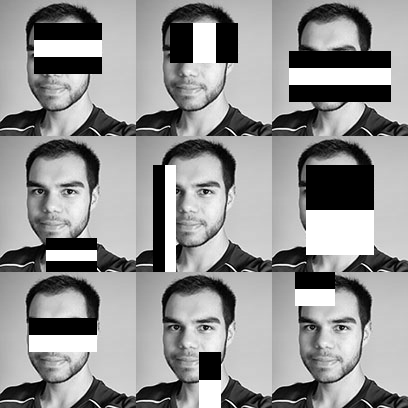
\includegraphics[height=0.6\textheight,width=\textwidth,keepaspectratio]{imagens/cascata_estagio_01.png}
    \end{subfigure}
    \begin{subfigure}[t]{0.24\textwidth}
    \centering
    \caption{Estágio 2}
    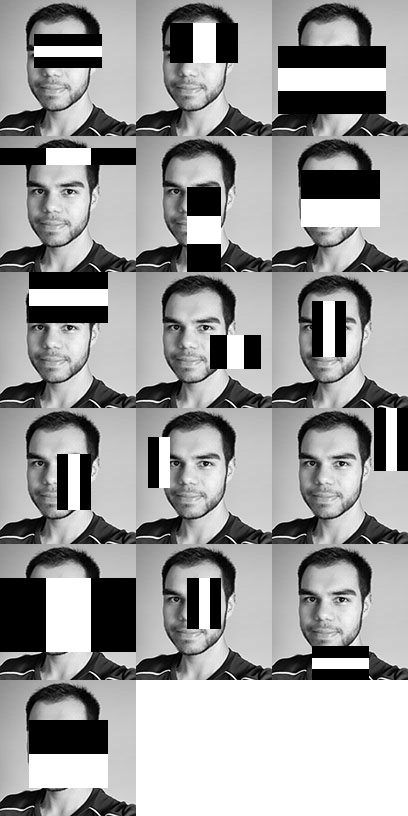
\includegraphics[height=0.6\textheight,width=\textwidth,keepaspectratio]{imagens/cascata_estagio_02.png}
    \end{subfigure}
    \begin{subfigure}[t]{0.24\textwidth}
    \centering
    \caption{Estágio 3}
    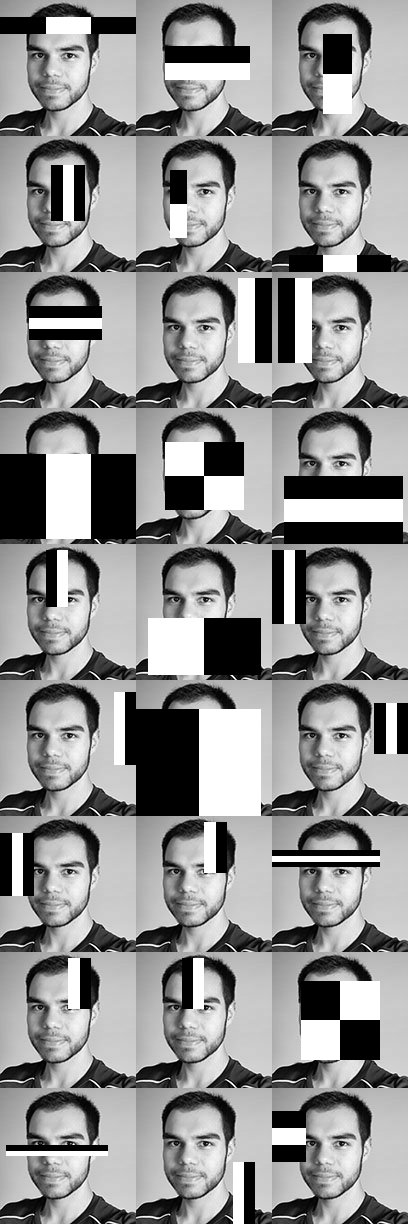
\includegraphics[height=0.6\textheight,width=\textwidth,keepaspectratio]{imagens/cascata_estagio_03.png}
    \end{subfigure}
    \begin{subfigure}[t]{0.24\textwidth}
    \centering
    \caption{Estágio 4}
    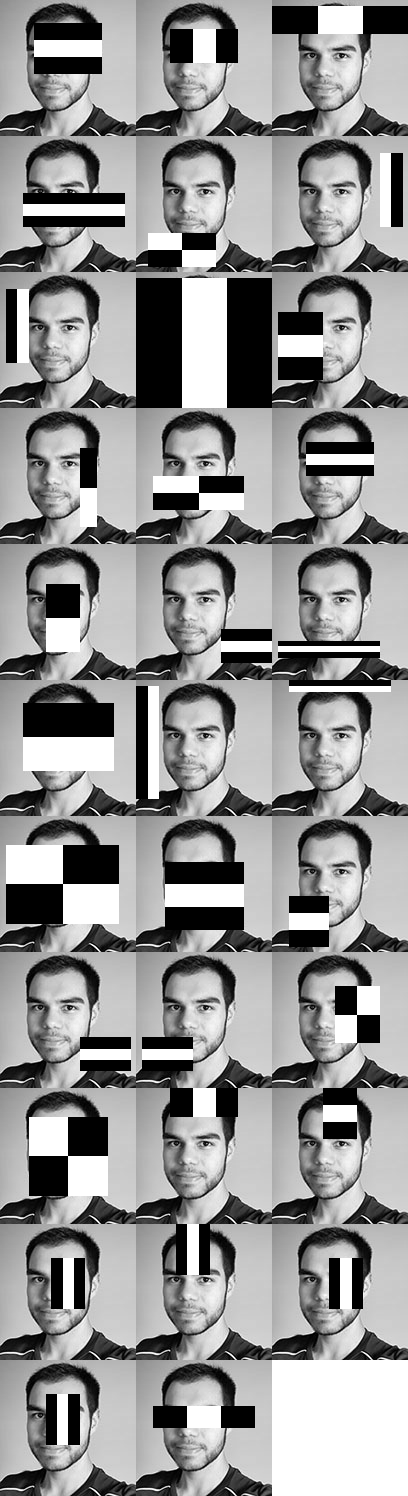
\includegraphics[height=0.6\textheight,width=\textwidth,keepaspectratio]{imagens/cascata_estagio_04.png}
    \end{subfigure}
\end{figure}
\end{frame}

%FRAME%%%%%%%%%%%%%%%%%%%%%%%%%%%%%%%%%%%%%%%%%%%%%%%
\begin{frame}{Classificadores em Cascata}
\begin{center}
\includemedia[
width=288px,
height=162px,
activate=pageopen,
addresource=imagens/VJ_detection-288x162.mp4,
flashvars={source=imagens/VJ_detection-288x162.mp4},
passcontext
]{}{VPlayer.swf}
\end{center}
\end{frame}

%FRAME%%%%%%%%%%%%%%%%%%%%%%%%%%%%%%%%%%%%%%%%%%%%%%%
\begin{frame}{FDDB Benchmark}
\begin{figure}
    \centering
    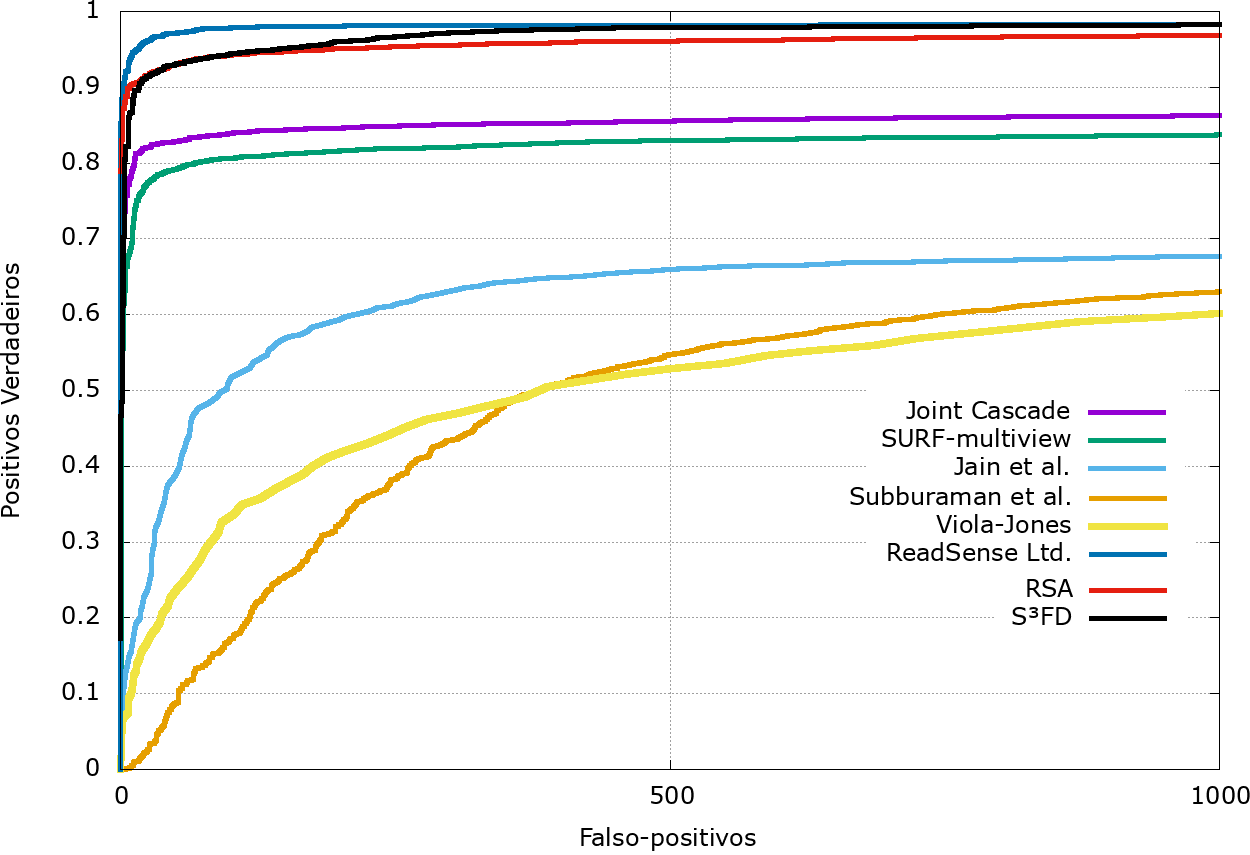
\includegraphics[height=0.82\textheight,width=\textwidth,keepaspectratio]{imagens/FDDB_deteccao_compara.png}
\end{figure}
\end{frame}


%SUBSEC%%%%%%%%%%%%%%%%%%%%%%%%%%%%%%%%%%%%%%%%%%%%%%%
\subsection{OpenCV}

%FRAME%%%%%%%%%%%%%%%%%%%%%%%%%%%%%%%%%%%%%%%%%%%%%%%
\begin{frame}{OpenCV}
Treinamento do classificador em cascata usando \texttt{opencv\_traincascade}:

\begin{itemize}
    \item 10 estágios
    \item 5000 imagens positivas
    \item 3000 imagens negativas
    \item 36$\times$36 pixels
    \item 99,5\% de detecção
    \item No máximo 50\% de falso-positivos por estágio
    \item Concluído em 1 dia 7 horas e 42 minutos
\end{itemize}

\end{frame}


%FRAME%%%%%%%%%%%%%%%%%%%%%%%%%%%%%%%%%%%%%%%%%%%%%%%
\begin{frame}[fragile]{OpenCV}
\begin{minted}[fontsize=\scriptsize]{python}
import cv2

classificador = cv2.CascadeClassifier('haarcascade_frontalface.xml')
camera = cv2.VideoCapture(0)

while camera.isOpened():
    _, imagem = camera.read()

    cinza = cv2.cvtColor(imagem, cv2.COLOR_BGR2GRAY)

    faces = classificador.detectMultiScale(
        cinza, scaleFactor=1.2, minNeighbors=5, minSize=(30, 30))

    for (x, y, w, h) in faces:
        cv2.rectangle(imagem, (x, y), (x + w, y + h), (0, 0, 255), 2)

    cv2.imshow('Detector de Faces', imagem)
\end{minted}
\end{frame}


%FRAME%%%%%%%%%%%%%%%%%%%%%%%%%%%%%%%%%%%%%%%%%%%%%%%
\begin{frame}{OpenCV}
Teste com imagens da Labeled Faces in the Wild
\begin{figure}[htbp]
%    \caption{Teste do classificador em cascata com imagens da Labeled Faces in the Wild}
    \label{fig:detector_facial_lfw}
    \begin{center}
        {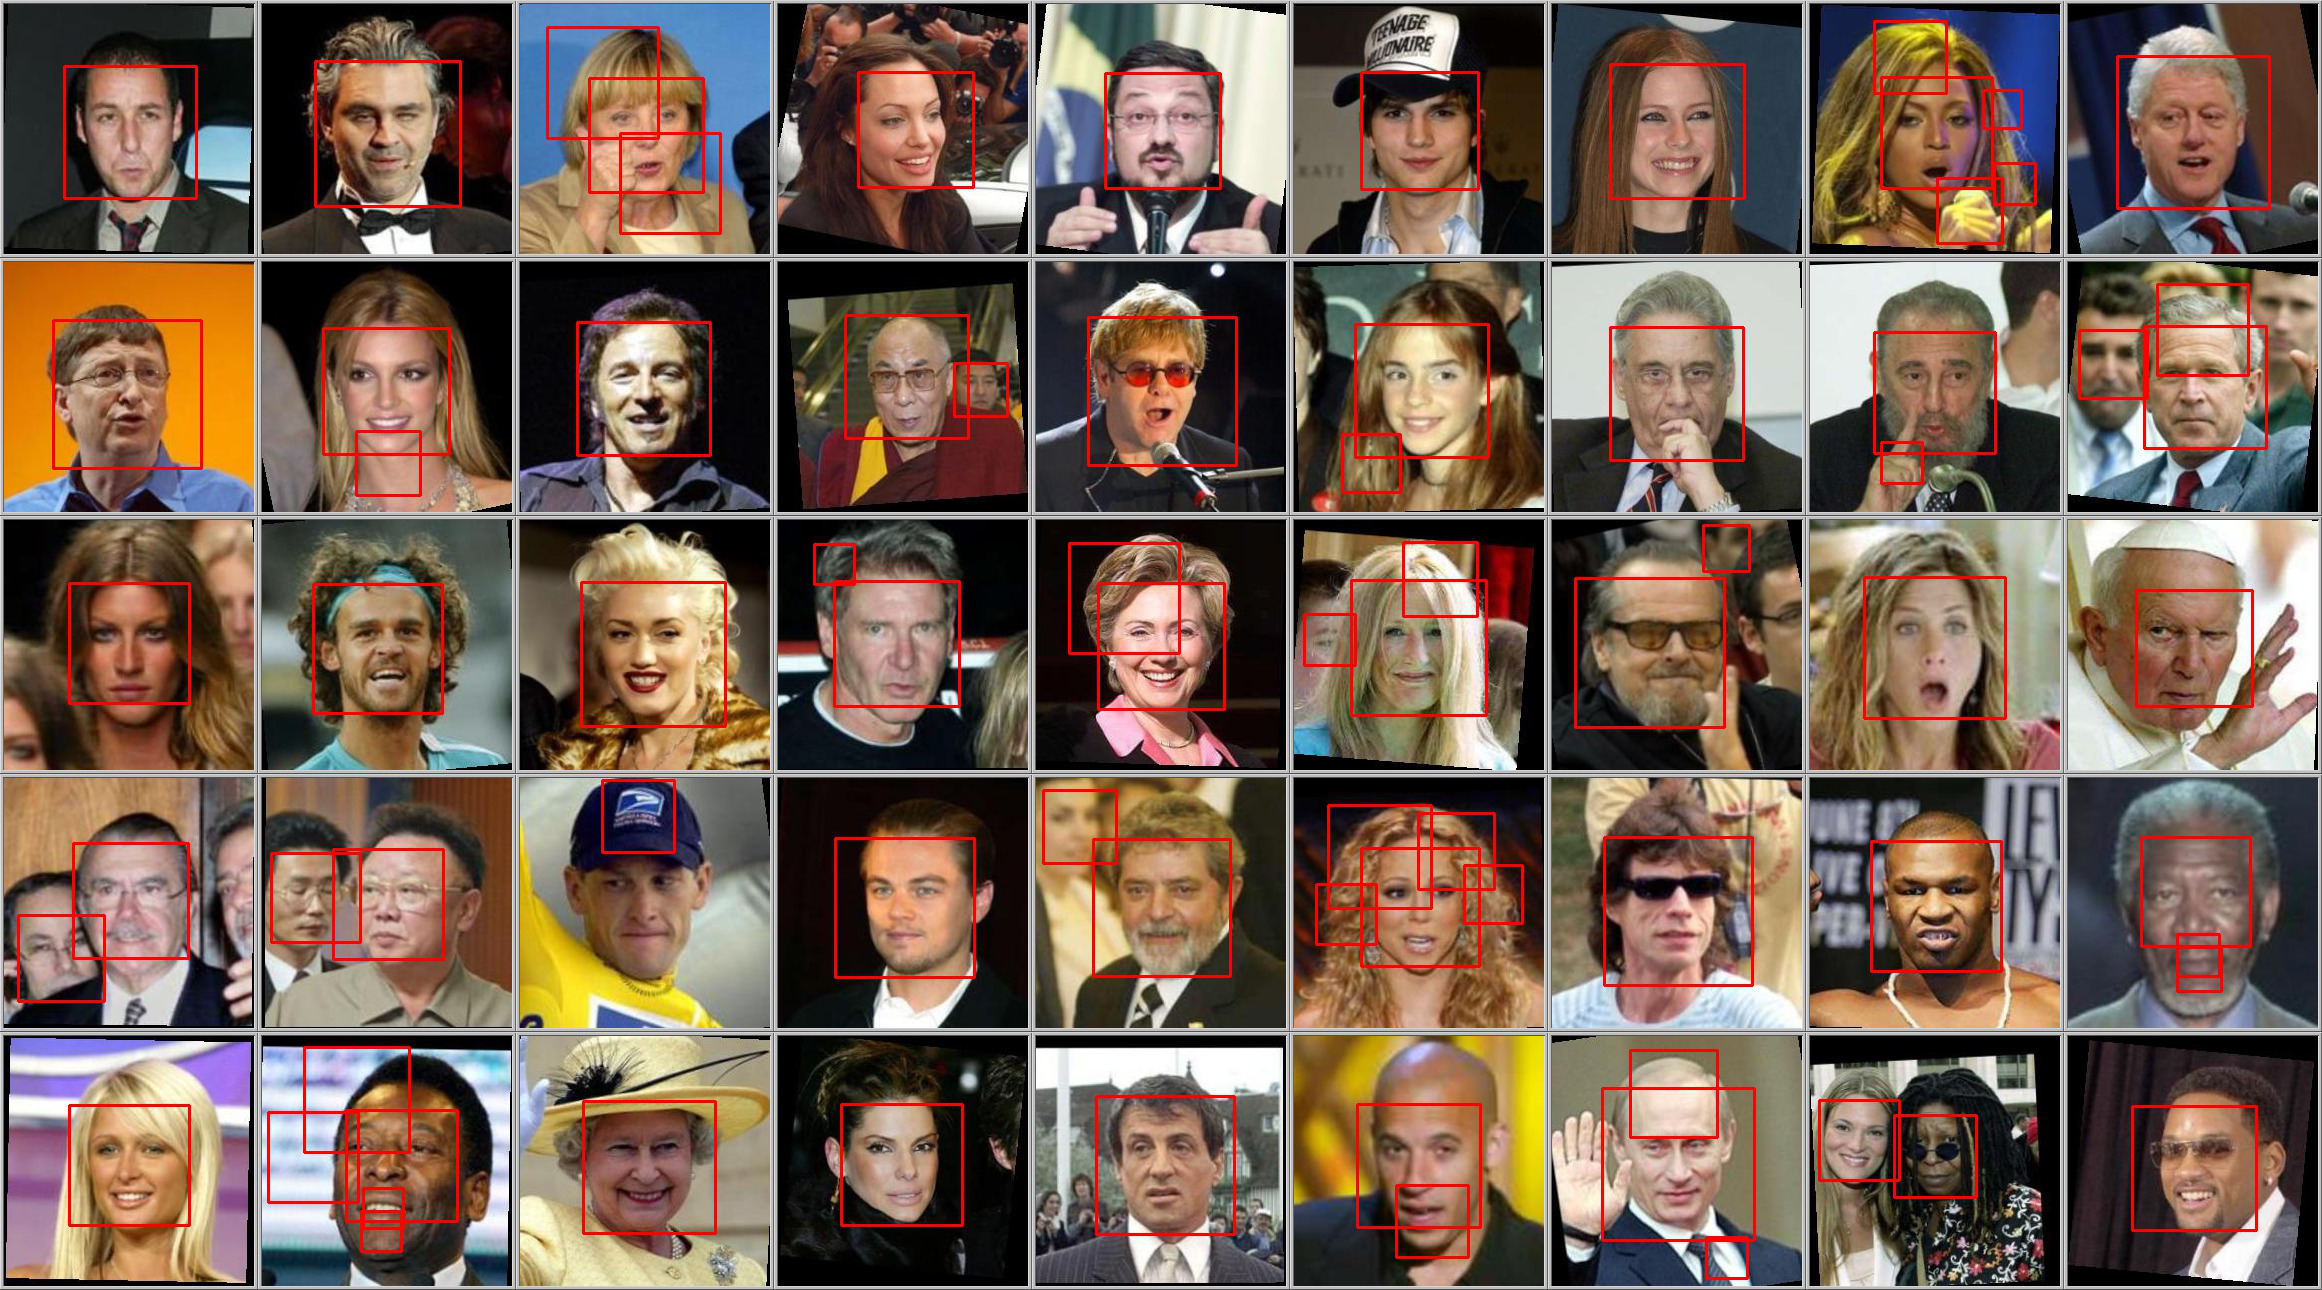
\includegraphics[width=0.99\linewidth]{imagens/detector_facial_lfw.jpg}}
    \end{center}
\end{figure}
\end{frame}